\documentclass[border=6pt]{standalone}
\usepackage{iftex}
% Use native SVG specials for the site's latex -> DVI -> SVG build.
% A normal pdflatex run still produces a standalone PDF for print.
\ifPDFTeX
  \ifnum\pdfoutput=0
    \def\pgfsysdriver{pgfsys-dvisvgm.def}
  \fi
\fi
\usepackage{tikz,amsmath}
\usetikzlibrary{arrows.meta}

\begin{document}
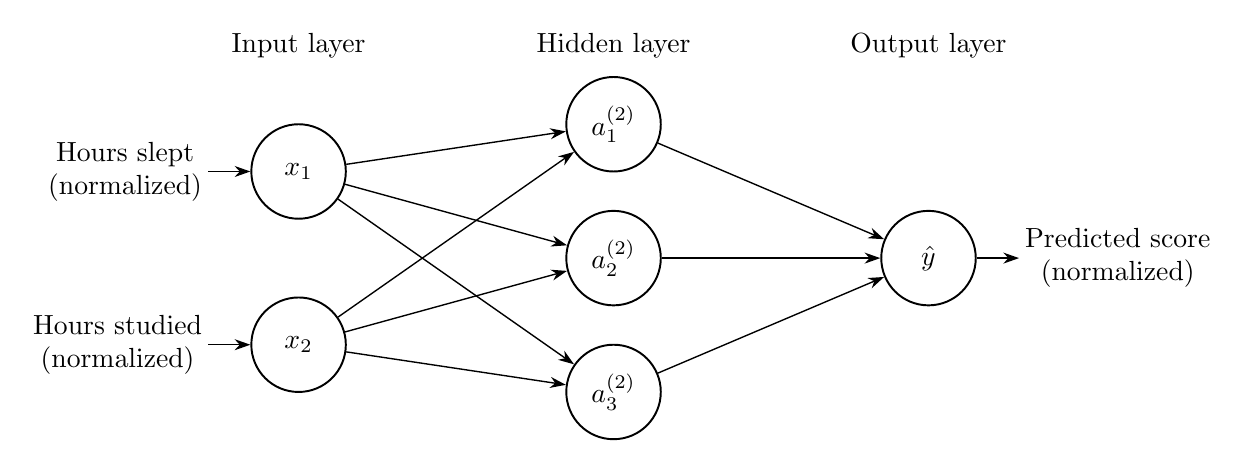
\begin{tikzpicture}[
  font=\normalsize,
  neuron/.style={circle, draw, line width=0.7pt, minimum size=12mm, inner sep=0pt},
  connection/.style={-{Stealth[length=2mm, width=1.4mm]}, line width=0.5pt},
  label/.style={align=center, inner sep=2pt}
]
  % The implemented network has two inputs, three hidden units, one output,
  % and no bias nodes. Labels refer to one example, with its row index omitted.
  \node[label] at (0,2.7) {Input layer};
  \node[label] at (4,2.7) {Hidden layer};
  \node[label] at (8,2.7) {Output layer};

  \node[neuron] (input1) at (0,1.1) {$x_1$};
  \node[neuron] (input2) at (0,-1.1) {$x_2$};

  \foreach \j/\y in {1/1.7, 2/0, 3/-1.7} {
    \node[neuron] (hidden\j) at (4,\y) {$a^{(2)}_{\j}$};
  }
  \node[neuron] (output) at (8,0) {$\hat{y}$};

  % Six input-to-hidden weights and three hidden-to-output weights.
  \foreach \i in {1,2} {
    \foreach \j in {1,2,3} {
      \draw[connection] (input\i) -- (hidden\j);
    }
  }
  \foreach \j in {1,2,3} {
    \draw[connection] (hidden\j) -- (output);
  }

  \node[label, anchor=east] (sleep) at (-1.15,1.1) {Hours slept\\(normalized)};
  \node[label, anchor=east] (study) at (-1.15,-1.1) {Hours studied\\(normalized)};
  \draw[connection] (sleep.east) -- (input1.west);
  \draw[connection] (study.east) -- (input2.west);

  \node[label, anchor=west] (prediction) at (9.15,0) {Predicted score\\(normalized)};
  \draw[connection] (output.east) -- (prediction.west);
\end{tikzpicture}
\end{document}
